\documentclass[12pt]{article}
\usepackage[margin=2.5cm]{geometry}
\usepackage{enumerate}
\usepackage{amsfonts}
\usepackage{amsmath}
\usepackage{fancyhdr}
\usepackage{amsmath}
\usepackage{amssymb}
\usepackage{amsthm}
\usepackage{mdframed}
\usepackage{graphicx}
\usepackage{subcaption}
\usepackage{adjustbox}
\usepackage{listings}
\usepackage{xcolor}
\usepackage{booktabs}
\usepackage[utf]{kotex}
\usepackage{hyperref}
\usepackage{accents}

\definecolor{codegreen}{rgb}{0,0.6,0}
\definecolor{codegray}{rgb}{0.5,0.5,0.5}
\definecolor{codepurple}{rgb}{0.58,0,0.82}
\definecolor{backcolour}{rgb}{0.95,0.95,0.92}

\lstdefinestyle{mystyle}{
    backgroundcolor=\color{backcolour},
    commentstyle=\color{codegreen},
    keywordstyle=\color{magenta},
    numberstyle=\tiny\color{codegray},
    stringstyle=\color{codepurple},
    basicstyle=\ttfamily\footnotesize,
    breakatwhitespace=false,
    breaklines=true,
    captionpos=b,
    keepspaces=true,
    numbers=left,
    numbersep=5pt,
    showspaces=false,
    showstringspaces=false,
    showtabs=false,
    tabsize=1
}

\lstset{style=mystyle}

\pagestyle{fancy}
\renewcommand{\headrulewidth}{0.4pt}
\lhead{CSC 343}
\rhead{Worksheet 8 Solution}

\begin{document}
\title{CSC343 Worksheet 8 Solution}
\maketitle

\bigskip

\begin{enumerate}[1.]
    \item

    \bigskip

    \begin{enumerate}[a)]
        \item

    \begin{lstlisting}[language=c]
    #include <float.h>

    #include sqlcli.h

    void askUserForPrice() {

        float targetPrice, minDiff, speedSol, minDiff = FLT_MAX;
        int modelSol;
        char makerSol;

        SQLHENV myEnv;
        SQLHDBC myCon;
        SQLHSTMT execStat;

        SQLINTEGER model, modelInfo, speedInfo, ram, ramInfo, hd, hdInfo, priceInfo, makerInfo;
        SQLREAL speed, price;
        SQLCHAR maker;


        errorCode1 = SQLAllocHandle(SQL_HANDLE_ENV,
                    SQL_NULL_HANDLE, &myEnv);

        if (!errorCode1) {
            errorCode2 = SQLAllocHandle(SQL_HANDLE_DBC, myEnv, &myCon);
        }

        if (!errorCode2) {
            errorCode3 = SQLAllocHandle(SQL_HANDLE_STMT, myCon, &execStat)
        }

        if (!errorCode3) {
            SQLPrepare(execStat,
                      "SELECT model, speed, ram, hd, price, maker "
                      "FROM Product NATURAL JOIN PC", SQL_NTS);
            SQLExecute(execStat);
            SQLBindCol(execStat, 1, SQL_INTEGER, &model, sizeof(model), &modelInfo);
            SQLBindCol(execStat, 2, SQL_FLOAT, &speed, sizeof(speed), &speedInfo);
            SQLBindCol(execStat, 3, SQL_INTEGER, &ram, sizeof(ram), &ramInfo);
            SQLBindCol(execStat, 4, SQL_INTEGER, &hd, sizeof(hd), &hdInfo);
            SQLBindCol(execStat, 5, SQL_FLOAT, &price, sizeof(price), &priceInfo);
            SQLBindCol(execStat, 6, SQL_CHAR, &maker, sizeof(maker), &makerInfo);

            printf("Enter target price:");
            scanf("%f", &targetPrice);

            while (SQLFetch(execStat) != SQL_NO_DATA) {

                if (abs(price - targetPrice) >= minDiff) {
                    continue;
                }

                minDiff = abs(price - targetPrice);
                modelSol = model;
                speedSol = speed;
                makerSol = maker;
            }

            printf("maker=%c, model=%d, speed=%.2f\n", makerSol, modelSol, speedSol);

        }
    }
    \end{lstlisting}

        \bigskip

        \underline{\textbf{Notes:}}

        \begin{itemize}
            \item Using Call-Level Interface
            \begin{itemize}
                \item Uses host language to connect to and access a database
                \item Replaces embedded SQL
            \end{itemize}
            \item Standard SQL/CLI
            \begin{itemize}
                \item Is database CLI for C
                \item Included in file \textit{sqlcli.h}
                \item Creates deals with four kinds of records

                \bigskip

                \begin{enumerate}[1.]
                    \item Environment handle
                    \begin{itemize}
                        \item Prepares one or more connections to database server
                        \item Is required
                        \item Is allocated using \textbf{SQLHENV}
                        \item Is established via function \textbf{SQLAllocHandle}

                        \begin{center}
                        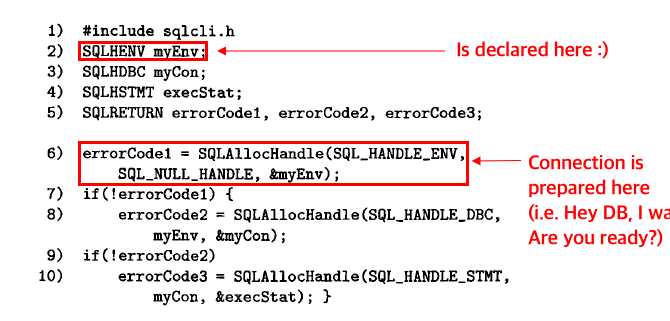
\includegraphics[width=\linewidth]{images/worksheet_8_solution_1.png}
                        \end{center}

                    \end{itemize}
                    \item Connection handle
                    \begin{itemize}
                        \item Conenects application program to database
                        \item Is required
                        \item Is declared after \textbf{SQLHENV}
                        \item Is allocated using \textbf{SQLHDBC}
                        \item Is established via function \textbf{SQLAllocHandle}

                        \begin{center}
                        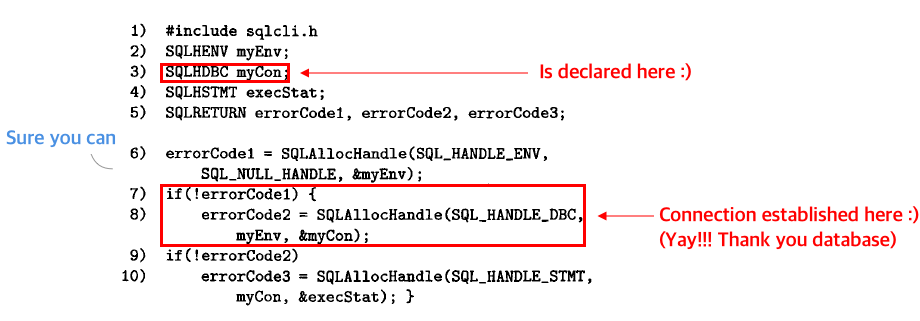
\includegraphics[width=\linewidth]{images/worksheet_8_solution_2.png}
                        \end{center}
                    \end{itemize}
                    \item Statements
                    \begin{itemize}
                        \item Created by application program (the user)
                        \item Can be created as many as needed
                        \item Holds information about a single SQL statement, including cursor
                        \item Can represent different SQL statements at different times
                        \item Is required
                        \item Is declared after \textbf{SQLHDBC}
                        \item Is allocated using \textbf{SQLHSTMT}
                        \item Is sent using the function \textbf{SQLAllocHandle}

                        \begin{center}
                        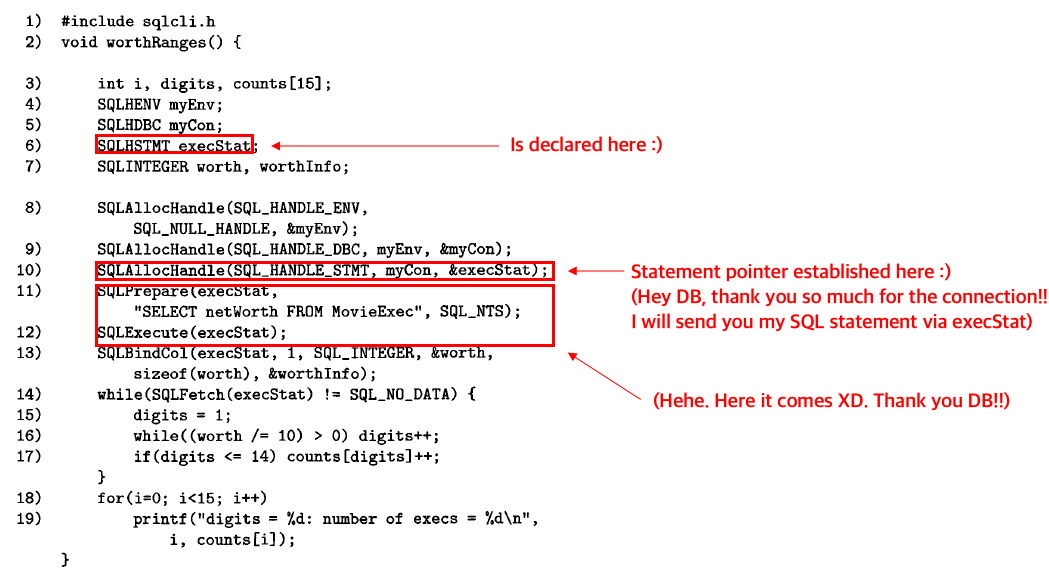
\includegraphics[width=\linewidth]{images/worksheet_8_solution_3.png}
                        \end{center}
                    \end{itemize}
                    \item Descriptions
                    \begin{itemize}
                        \item Holds information about either tuples or parameters
                        \item Each statement has this information implicitly
                    \end{itemize}
                \end{enumerate}
            \end{itemize}
            \item Processing Statements
            \begin{itemize}
                \item is done using \textbf{SQLPrepare} and \textbf{SQLExecute}

                \begin{align}
                    \textbf{SQLPrepare}(sh,st,SQL\_NTS)\\
                    \textbf{SQLExecute}(sh)
                \end{align}

                \item $sh$ is the statement handle created using \textbf{SQLHSTMT}
                \item SQL\_NTS evaluates the length of string in $st$

                \bigskip

                \underline{\textbf{Example:}}

                \bigskip

    \begin{lstlisting}[language=c]
    SQLPrepare(execStat, "SELECT netWorth FROM MovieExec", SQL_NTS);
    SQLExecute(execStat);
    \end{lstlisting}
                \item the function \textbf{SQLExecDirect} combines \textbf{SQLPrepare} and \textbf{SQLExecute}

                \bigskip

                \underline{\textbf{Example 2:}}

                \bigskip

    \begin{lstlisting}[language=c]
    SQLExecDirect(execStat, "SELECT netWorth FROM MovieExec", SQL_NTS);
    \end{lstlisting}
            \end{itemize}
            \item Fetching Data From
            \begin{itemize}
                \item Fetch
                \begin{itemize}
                    \item \textbf{Syntax:} SQLFetch(sh)
                    \item Executes statement in \textbf{SQLPrepare} and \textbf{SQLExecute} and stores result
                    to variable in \textbf{SQLBindCol}
                    \item Fetches a row per call
                    \item Returns a value of type \textbf{SQLRETURN}, indicating either success or error
                \end{itemize}
                \item SQLBindCol
                \begin{itemize}
                    \item \textbf{Syntax:} $\text{SQLBindCol}(sh, colNo, colType, pVar, varSize, varInfo)$
                    \begin{itemize}
                        \item \textbf{sh}: the handle of statement (e.g execStat)
                        \item \textbf{colNo}: the position of column in tuple we obtain
                        \item \textbf{colType}: the SQL data type of variable (e.g. SQL\_INTEGER, SQL\_CHAR)
                        \item \textbf{pVar}: the pointer to variable the value is placed
                        \item \textbf{varSize}: the length in bytes of the value in $pVar$
                        \item \textbf{varInfo}: a pointer to an integer used by SQLBindCol for additional value
                        about the value produced
                    \end{itemize}
                    \item Stores data from \textbf{SQLFetch} to host-language variable
                    \item Must be setup before SQLFetch(sh) is run
                \end{itemize}
            \end{itemize}

            \begin{center}
            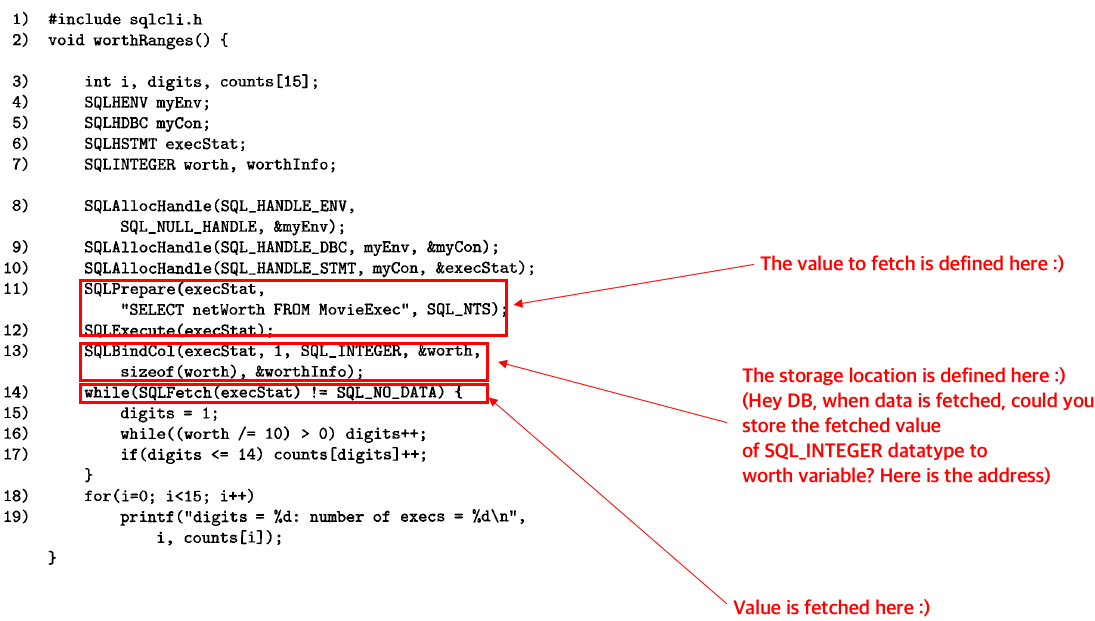
\includegraphics[width=\linewidth]{images/worksheet_8_solution_4.png}
            \end{center}
        \end{itemize}

        \item

    \begin{lstlisting}[language=c]
    #include sqlcli.h

    void findLaptops() {

        float minSpeed, minPrice;
        int minRam, minHd;

        SQLINTEGER model, modelInfo, speedInfo, ram, ramInfo, hd, hdInfo, priceInfo, makerInfo, screen, screenInfo;
        SQLREAL speed, price;
        SQLCHAR maker;

        errorCode1 = SQLAllocHandle(SQL_HANDLE_ENV,
                    SQL_NULL_HANDLE, &myEnv);

        if (!errorCode1) {
            errorCode2 = SQLAllocHandle(SQL_HANDLE_DBC, myEnv, &myCon);
        }

        if (!errorCode2) {
            errorCode3 = SQLAllocHandle(SQL_HANDLE_STMT, myCon, &execStat)
        }

        if (!errorCode3) {
            SQLPrepare(execStat,
                      "SELECT model, speed, ram, hd, screen, price, maker "
                      "FROM Product NATURAL JOIN Laptop", SQL_NTS);
            SQLExecute(execStat);
            SQLBindCol(execStat, 1, SQL_INTEGER, &model, sizeof(model), &modelInfo);
            SQLBindCol(execStat, 2, SQL_FLOAT, &speed, sizeof(speed), &speedInfo);
            SQLBindCol(execStat, 3, SQL_INTEGER, &ram, sizeof(ram), &ramInfo);
            SQLBindCol(execStat, 4, SQL_INTEGER, &hd, sizeof(hd), &hdInfo);
            SQLBindCol(execStat, 5, SQL_INTEGER, &screen, sizeof(screen), &screenInfo);
            SQLBindCol(execStat, 6, SQL_FLOAT, &price, sizeof(price), &priceInfo);
            SQLBindCol(execStat, 7, SQL_CHAR, &maker, sizeof(maker), &makerInfo);

            printf("Enter minimum speed:");
            scanf("%f", &minSpeed);

            printf("Enter minimum ram:");
            scanf("%f", &minRam);

            printf("Enter minimum hard-drive space:");
            scanf("%f", &minHd);

            printf("Enter minimum price:");
            scanf("%f", &minPrice);

            while(SQLFetch(execStat) != SQL_NO_DATA) {
                if (
                    speed >= minSpeed &&
                    ram >= minRam &&
                    hd >= minHd &&
                    screen >= minScreen
                ) {
                    printf("model=%d, speed=%.2f, ram=%d, hd=%d, screen=%d, price=%.2f, maker=%c",
                        model, speed, ram, hd, screen, price, maker);
                }
            }
        }
    }
    \end{lstlisting}

        \item

    \begin{lstlisting}[language=c]
    #include <stdbool.h>
    #include <string.h>
    ...
    void printSpecifications() {
        char targetMaker;

        SQLHENV myEnv;
        SQLHDBC myCon;
        SQLHSTMT execStat, subExecStat;

        SQLINTEGER model, modelInfo, speedInfo, ram, ramInfo, hd, hdInfo, priceInfo, makerInfo, screen, screenInfo, color, colorInfo, printTypeInfo;
        SQLREAL speed, price;
        SQLCHAR maker, printType[50];

        SQLRETURN errorCode1, errorCode2, errorCode3;

        errorCode1 = SQLAllocHandle(SQL_HANDLE_ENV,
                    SQL_NULL_HANDLE, &myEnv);

        if (!errorCode1) {
            errorCode2 = SQLAllocHandle(SQL_HANDLE_DBC, myEnv, &myCon);
        }

        if (!errorCode2) {
            errorCode3 = SQLAllocHandle(SQL_HANDLE_STMT, myCon, &execStat);
            errorCode4 = SQLAllocHandle(SQL_HANDLE_STMT, myCon, &subExecStat);
        }

        if (!errorCode3 && !errorCode4) {
            printf("Enter manufacturer:");
            scanf("%c", &targetMaker);

            SQLBindCol(execStat, 1, SQL_CHAR, &maker, sizeof(maker), &makerInfo);
            SQLBindCol(execStat, 2, SQL_CHAR, &productType, sizeof(productType), &productTypeInfo);

            while (SQLFetch(execStat) != SQL_NO_DATA) {
                if (strcmp(productType,'pc')) {
                    SQLPrepare(subExecStat,
                                "SELECT speed, ram, hd, price FROM PC "
                                "NATURAL JOIN Product "
                                "WHERE type= ?", SQL_NTS);
                        SQLBindParameter(subExecStat, 1, ..., productType, ...);
                    SQLExecute(subExecStat);

                    SQLBindCol(subExecStat, 1, SQL_FLOAT, &speed, sizeof(speed), &speedInfo);
                    SQLBindCol(subExecStat, 2, SQL_INTEGER, &ram, sizeof(ram), &ramInfo);
                    SQLBindCol(subExecStat, 3, SQL_INTEGER, &hd, sizeof(hd), &hdInfo);
                    SQLBindCol(subExecStat, 4, SQL_FLOAT, &price, sizeof(price), &priceInfo);

                    while(SQLFetch(subExecStat) != SQL_NO_DATA) {
                        printf("model=%d, speed=%.2f, ram=%d, hd=%d, price=%.2f, maker=%c, type=%s",
                        model, speed, ram, hd, screen, price, maker, productType);
                    }
                } else if (strcmp(productType, 'laptop')) {

                    SQLPrepare(subExecStat,
                                "SELECT speed, ram, hd, screen, price FROM Laptop "
                                "NATURAL JOIN Product "
                                "WHERE type= ?", SQL_NTS);
                        SQLBindParameter(subExecStat, 1, ..., productType, ...);
                    SQLExecute(subExecStat);

                    SQLBindCol(subExecStat, 1, SQL_FLOAT, &speed, sizeof(speed), &speedInfo);
                    SQLBindCol(subExecStat, 2, SQL_INTEGER, &ram, sizeof(ram), &ramInfo);
                    SQLBindCol(subExecStat, 3, SQL_INTEGER, &hd, sizeof(hd), &hdInfo);
                    SQLBindCol(subExecStat, 4, SQL_INTEGER, &screen, sizeof(screen), &screenInfo);
                    SQLBindCol(subExecStat, 5, SQL_FLOAT, &price, sizeof(price), &priceInfo);

                    while(SQLFetch(subExecStat) != SQL_NO_DATA) {
                        printf("model=%d, speed=%.2f, ram=%d, hd=%d, screen=%d, price=%.2f, maker=%c, type=%s",
                        model, speed, ram, hd, screen, screen, price, maker, productType);
                    }
                } else if (strcmp(productType, 'printer')) {
                    SQLPrepare(subExecStat,
                                "SELECT color, printType, price FROM Printer "
                                "NATURAL JOIN Product "
                                "WHERE type= ?", SQL_NTS);
                        SQLBindParameter(subExecStat, 1, ..., productType, ...);
                    SQLExecute(subExecStat);

                    SQLBindCol(subExecStat, 1, SQL_INTEGER, &color, sizeof(speed), &speedInfo);
                    SQLBindCol(subExecStat, 2, SQL_CHAR, &printType, sizeof(printType), &printTypeInfo);
                    SQLBindCol(subExecStat, 3, SQL_FLOAT, &price, sizeof(price), &priceInfo);

                    while(SQLFetch(subExecStat) != SQL_NO_DATA) {
                        printf("model=%d, color=%s, price=%.2f, maker=%c, type=%s",
                        model, color ? "true" : "false", price, maker, type);
                    }
                }
            }
        }
    }
    \end{lstlisting}

        \item
        \item

    \begin{lstlisting}[language=c]
    #include <sqlcli.h>
    #include <string.h>
    ...
    void insertNewPC() {

        int model, ram, hd;
        float speed, price;
        char maker;

        SQLINTEGER modelCount;

        SQLHENV myEnv;
        SQLHDBC myCon;
        SQLHSTMT execStat, subExecStat;

        SQLRETURN errorCode1, errorCode2, errorCode3;

        errorCode1 = SQLAllocHandle(SQL_HANDLE_ENV,
                    SQL_NULL_HANDLE, &myEnv);

        if (!errorCode1) {
            errorCode2 = SQLAllocHandle(SQL_HANDLE_DBC, myEnv, &myCon);
        }

        if (!errorCode2) {
            errorCode3 = SQLAllocHandle(SQL_HANDLE_STMT, myCon, &execStat);
        }

        if (!errorCode3) {
            printf("Enter manufacturer:\n");
            scanf("%c", &maker);

            printf("Enter model:\n");
            scanf("%d", &model);

            printf("Enter speed:\n");
            scanf("%f", &speed);

            printf("Enter ram:\n");
            scanf("%d", &ram);

            printf("Enter hd:\n");
            scanf("%d", &hd);

            printf("Enter price:\n");
            scanf("%f", &price);

            printf("Enter maker:\n");
            scanf("%c", &maker);

            SQLPrepare(execStat,
                      "SELECT COUNT(model) FROM ("
                      "(SELECT model FROM Product WHERE model=:model) "
                      "UNION "
                      "(SELECT model FROM PC WHERE model= ?)", SQL_NTS);
                SQLBindParameter(execStat, 1, ..., model, ...);
            SQLExecute(execStat);
            SQLBindCol(execStat, 1, SQL_INT, &modelCount, sizeof(modelCount), &modelCountInfo);

            if (modelCount != 0) {
                printf("Error. Model already exists in database.");
            } else {
                SQLPrepare(execStat,
                        "INSERT INTO PC(model, speed, ram, hd, price)"
                        "VALUES(?, ?, ?, ?, ?)", SQL_NTS);
                    SQLBindParameter(execStat, 1, ..., model, ...);
                    SQLBindParameter(execStat, 2, ..., speed, ...);
                    SQLBindParameter(execStat, 3, ..., ram, ...);
                    SQLBindParameter(execStat, 4, ..., hd, ...);
                    SQLBindParameter(execStat, 5, ..., price, ...);
                SQLExecute(execStat);

                SQLPrepare(execStat,
                        "INSERT INTO Product(model, maker, type)"
                        "VALUES(?, ?, 'pc')", SQL_NTS);
                    SQLBindParameter(execStat, 1, ..., model, ...);
                    SQLBindParameter(execStat, 2, ..., maker, ...);
                SQLExecute(execStat);
            }
        }
    }
    \end{lstlisting}

    \end{enumerate}

    \item

    \begin{enumerate}[a)]
        \item

    \begin{lstlisting}[language=c]
    void classWithLargestPower() {

        SQLINTEGER classInfo;
        SQLCHAR class[100];

        SQLHENV myEnv;
        SQLHDBC myCon;
        SQLHSTMT execStat, subExecStat;

        SQLRETURN errorCode1, errorCode2, errorCode3;

        errorCode1 = SQLAllocHandle(SQL_HANDLE_ENV,
                    SQL_NULL_HANDLE, &myEnv);

        if (!errorCode1) {
            errorCode2 = SQLAllocHandle(SQL_HANDLE_DBC, myEnv, &myCon);
        }

        if (!errorCode2) {
            errorCode3 = SQLAllocHandle(SQL_HANDLE_STMT, myCon, &execStat);
        }

        if (!errorCode3) {
            SQLPrepare(execStat,
                      "SELECT class FROM FROM Classes"
                      "WHERE numGuns * POWER(bore, 3) >= ALL ( "
                      "SELECT numGuns * POWER(bore, 3) FROM Classes "
                      ")", SQL_NTS);
                SQLBindParameter(execStat, 1, ..., model, ...);
            SQLExecute(execStat);
            SQLBindCol(execStat, 1, SQL_CHAR, &class, sizeof(class), &classInfo);

            while(SQLFetch(execStat) != SQL_NO_DATA) {
                printf("Class = %s\n", class);
            }
        }
    }
    \end{lstlisting}

        \item

    \begin{lstlisting}[language=c]
    #include <sqlcli.h>
    #include <string.h>
    ...
    void countryWithMostShipsSunk() {
        char targetBattle[255];
        char mostSunkCountry[100];
        int maxSunkCount = 0, loopIndex = 0;

        char mostDamagedCountry[100];
        int maxDamagedCount = 0;

        SQLCHAR country[100];
        SQLINTEGER count, countInfo. countryInfo;

        SQLHENV myEnv;
        SQLHDBC myCon;
        SQLHSTMT execStat, subExecStat;

        SQLRETURN errorCode1, errorCode2, errorCode3;

        errorCode1 = SQLAllocHandle(SQL_HANDLE_ENV,
                    SQL_NULL_HANDLE, &myEnv);

        if (!errorCode1) {
            errorCode2 = SQLAllocHandle(SQL_HANDLE_DBC, myEnv, &myCon);
        }

        if (!errorCode2) {
            errorCode3 = SQLAllocHandle(SQL_HANDLE_STMT, myCon, &execStat)
        }

        if (!errorCode3) {

            printf("Enter name of battle:\n");
            scanf("%s", &targetBattle);

            SQLPrepare(execStat,
                        "SELECT country, COUNT(Outcomes.result) FROM Classes "
                        "INNER JOIN Ships ON Classes.class = Ships.class "
                        "INNER JOIN Outcomes ON Ships.name = Outcomes.ship "
                        "INNER JOIN Battles ON Battles.name = Outcome.battle "
                        "GROUP BY country "
                        "HAVING Battles.name=:targetBattle AND"
                        "Outcomes.result='sunk'", SQL_NTS);
            SQLExecute(execStat);
            SQLBindCol(execStat, 1, SQL_CHAR, &country, sizeof(country), &countryInfo);
            SQLBindCol(execStat, 2, SQL_INTEGER, &count, sizeof(count), &countInfo);

            while(SQLFetch(execStat) != SQL_NO_DATA) {
                if (loopIndex == 0) {
                    strcpy(mostSunkCountry, country);
                }

                if (count > maxSunkCount) {
                    maxSunkCount = count;
                    strcpy(mostSunkCountry, country);
                }
                loopIndex = loopIndex + 1;
            }

            printf("Country with most sunk ships: %s", mostSunkCountry);


            count = 0;
            loopIndex = 0;
            SQLPrepare(execStat,
                        "SELECT country, COUNT(Outcomes.result) FROM Classes "
                        "INNER JOIN Ships ON Classes.class = Ships.class "
                        "INNER JOIN Outcomes ON Ships.name = Outcomes.ship "
                        "INNER JOIN Battles ON Battles.name = Outcome.battle "
                        "GROUP BY country "
                        "HAVING Battles.name=:targetBattle AND"
                        "Outcomes.result='damaged'", SQL_NTS);
            SQLExecute(execStat);

            while(SQLFetch(execStat) != SQL_NO_DATA) {
                if (loopIndex == 0) {
                    strcpy(mostDamagedCountry, country);
                }

                if (count > maxDamagedCount) {
                    maxDamagedCount = count;
                    strcpy(mostDamagedCountry, country);
                }
                loopIndex = loopIndex + 1;
            }

            printf("Country with most damaged ships: %s", mostDamagedCountry);
        }
    }
    \end{lstlisting}

        \item

    \begin{lstlisting}[language=c]
    #include <sqlcli.h>

    void insertClassAndShip() {

        char class[100], type[2], country[100], shipName[100], dateLaunched[11];
        int numGuns, bore, displacement;


        SQLHENV myEnv;
        SQLHDBC myCon;
        SQLHSTMT execStat, subExecStat;

        SQLRETURN errorCode1, errorCode2, errorCode3;

        errorCode1 = SQLAllocHandle(SQL_HANDLE_ENV,
                    SQL_NULL_HANDLE, &myEnv);

        if (!errorCode1) {
            errorCode2 = SQLAllocHandle(SQL_HANDLE_DBC, myEnv, &myCon);
        }

        if (!errorCode2) {
            errorCode3 = SQLAllocHandle(SQL_HANDLE_STMT, myCon, &execStat)
        }

        if (!errorCode3) {
            printf("Enter name of class:\n");
            scanf("%s", class);

            printf("Enter name of type ('bb' or 'bc'):\n");
            scanf("%s", type);

            printf("Enter name of country:\n");
            scanf("%s", country);

            printf("Enter name of numGuns:\n");
            scanf("%d", &numGuns);

            printf("Enter name of bore:\n");
            scanf("%d", &bore);

            printf("Enter name of displacement:\n");
            scanf("%d", &displacement);

            printf("Enter name of ship (if first ship, skip by pressing ENTER):\n");
            fgets(shipName, sizeof shipName,stdin);

            if (shipName[0] == '\n') {
                strncpy(shipName, class, sizeof(class));
            }

            printf("Enter date launched (YYYY-MM-DD):\n");
            scanf("%s", dateLaunched);

            SQLPrepare(execStat,
                    "INSERT INTO Classes(class, type, country, numGuns, bore, displacement)"
                    "VALUES (?, ?, ?, ?, ?, ?)", SQL_NTS);
                SQLBindParameter(execStat, 1, ..., class, ...);
                SQLBindParameter(execStat, 2, ..., type, ...);
                SQLBindParameter(execStat, 3, ..., country, ...);
                SQLBindParameter(execStat, 4, ..., numGuns, ...);
                SQLBindParameter(execStat, 5, ..., bore, ...);
                SQLBindParameter(execStat, 6, ..., displacement, ...);
            SQLExecute(execStat);

            SQLPrepare(execStat,
                    "INSERT INTO Ships(name, class, launched)"
                    "VALUES (?, ?, ?)", SQL_NTS);
                SQLBindParameter(execStat, 1, ..., shipName, ...);
                SQLBindParameter(execStat, 2, ..., class, ...);
                SQLBindParameter(execStat, 3, ..., dateLaunched, ...);
            SQLExecute(execStat);
        }
    }
    \end{lstlisting}

        \item

    \begin{lstlisting}[language=c]
    #include <sqlcli.h>

    void correctError() {
        SQLCHAR battle[101], shipName[101];
        DATE_STRUCT dateLaunched;
        DATE_STRUCT dateBattle;

        int newDateLaunchedDay;
        int newDateLaunchedMonth;
        int newDateLaunchedYear;

        int newDateBattleDay;
        int newDateBattleMonth;
        int newDateBattleYear;

        SQLCHAR name[101], class[101]

        SQLHENV myEnv;
        SQLHDBC myCon;
        SQLHSTMT execStat, subExecStat;

        SQLRETURN errorCode1, errorCode2, errorCode3, errorCode4;

        errorCode1 = SQLAllocHandle(SQL_HANDLE_ENV,
                    SQL_NULL_HANDLE, &myEnv);

        if (!errorCode1) {
            errorCode2 = SQLAllocHandle(SQL_HANDLE_DBC, myEnv, &myCon);
        }

        if (!errorCode2) {
            errorCode3 = SQLAllocHandle(SQL_HANDLE_STMT, myCon, &execStat);
            errorCode4 = SQLAllocHandle(SQL_HANDLE_STMT, myCon, &subExecStat);
        }

        if (!errorCode3 && !errorCode4) {

            SQLPrepare(execStat,
                        "SELECT Ships.name, Ships.class, Outcomes.battle"
                        "FROM Ships "
                        "INNER JOIN Outcomes ON Ships.name = Outcomes.ship "
                        "INNER JOIN Battles ON Outcomes.battle = Battles.name "
                        "WHERE Ships.launched > Battles.date", SQL_NTS);
            SQLExecute(execStat);
            SQLBindCol(execStat, 1, SQL_CHAR, &shipName, sizeof(shipName), &shipNameInfo);
            SQLBindCol(execStat, 2, SQL_FLOAT, &class, sizeof(class), &classInfo);
            SQLBindCol(execStat, 3, SQL_INTEGER, &battle, sizeof(battle), &battleInfo);

            while(SQLFetch(execStat) != SQL_NO_DATA) {

                printf("Error. Ship %s is launched after date of battle.\n");

                printf("Enter correct launched date (YYYY-MM-DD. Type 0-0-0 to skip):\n");
                scanf("%d-%d-%d", &newDateLaunchedDay, &newDateLaunchedMonth, &newDateLaunchedYear);

                if (!newDateLaunchedDay == 0 &&
                    !newDateLaunchedMonth == 0 &&
                    !newDateLaunchedYear == 0) {
                    // Correct date of launch
                    SQLPrepare(subExecStat,
                                "UPDATE Ships "
                                "SET launched = ? "
                                "WHERE name = ? AND class = ?", SQL_NTS);
                        SQLBindParameter(subExecStat, 1, ..., newDateLaunched, ...);
                        SQLBindParameter(subExecStat, 2, ..., shipName, ...);
                        SQLBindParameter(subExecStat, 3, ..., class, ...);
                    SQLExecute(subExecStat);
                }

                printf("Enter correct launched date (YYYY-MM-DD. Type 0-0-0 to skip):\n");
                scanf("%d-%d-%d", &newDateBattleDay, &newDateBattleMonth, &newDateBattleYear);

                if (!newDateBattleDay == 0 &&
                    !newDateBattleMonth == 0 &&
                    !newDateBattleYear == 0) {
                    // Correct date of battle
                    SQLPrepare(subExecStat,
                                "UPDATE Battles "
                                "SET date = ? "
                                "WHERE name = ?", SQL_NTS);
                        SQLBindParameter(subExecStat, 1, ..., newDateBattle, ...);
                        SQLBindParameter(subExecStat, 2, ..., battle, ...);
                    SQLExecute(subExecStat);
                }
            }
        }
    }
    \end{lstlisting}

    \end{enumerate}

    \item

    \begin{enumerate}[a)]
        \item

        \bigskip

        \underline{\textbf{Notes:}}

        \bigskip

        \begin{itemize}
            \item JDBC
            \begin{itemize}
                \item Setup

                \bigskip

                \begin{enumerate}[1.]
                    \item Import JDBC

                    \bigskip

                    import java.sql.*;

                    \bigskip

                    \item Load a drive rfor the database system to use (i.e. sqlite, postgresql, mysql)

                    \bigskip

                    Class.forName($<\text{driver name}>$);

                    \bigskip

                    \underline{\textbf{Example:}}

                    \bigskip

                    Class.forName("com.mysql.jdbc.Driver");

                    \bigskip

                    \item Establish a connection to the database

                    \bigskip

                    Connection myCon = DriverManager.getConnection($<\text{URL}>$, $<\text{user name}>$, $<\text{password}>$);

                    \begin{itemize}
                        \item The url for jdbc is

                        \bigskip

                        jdbc:mysql://$<\text{host name}>$/$<\text{database name}>$

                        \bigskip
                    \end{itemize}

                \end{enumerate}
                \item Creating Statements in JDBC
                \item Cursor Operations in JDBC
                \item Parameter Passing
            \end{itemize}
        \end{itemize}
    \end{enumerate}

\end{enumerate}

\end{document}